% vim: ft=tex cc=79 ts=3 sw=3 et
% 
% iframe = master frame; pframe = slave frame
\iframe{Философия UNIX}

Write programs that do one thing and do it well.
Write programs to work together.
Write programs to handle text streams, because that is a universal interface.
\\ \hfill Peter H. Salus.

\pause

Clarity is better than cleverness.
In interface design, always do the least surprising thing.
When a program has nothing surprising to say, it should say nothing.
\\ \hfill Eric S. Raymond.

\vfill

\small
\hspace{-0.2cm}\url{http://catb.org/esr/writings/taoup/html/ch01s06.html}

\end{frame}

\pframe{Принцип KISS}

\centering
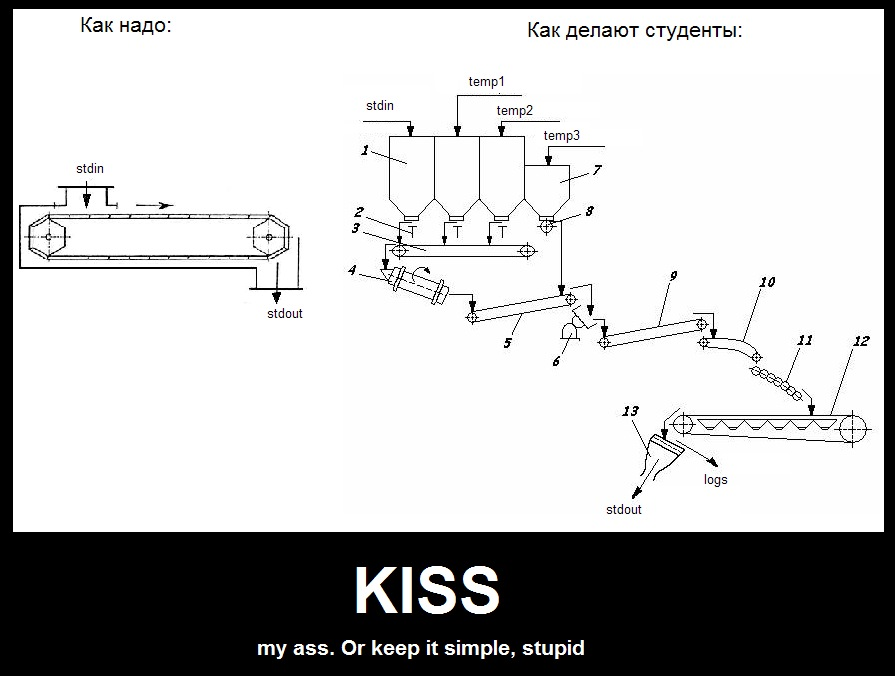
\includegraphics[width=0.9\textwidth]{img/kiss.jpg}

\end{frame}
